\documentclass{article}
\usepackage[utf8]{inputenc}
\usepackage[a4paper, total={6.4in, 8.53in}]{geometry}
\usepackage{amsmath, tikz, amsfonts, bbm, mathrsfs, graphicx, amssymb, amsthm, hyperref, centernot, enumerate, bbm, xcolor, lmodern, mathdots, amsfonts, graphicx, subcaption, booktabs, array}

\title{MAT1856/APM466 Assignment 1}
\author{Ruizi Liu, Student \#: 1008238275}
\date{February, 2025}

\begin{document}

\maketitle

\section*{Fundamental Questions - 25 points}

\begin{enumerate}
    \item \hfill
    \begin{enumerate}
        \item Governments issue bonds instead of printing money to control inflation, stabilize the economy, manage interest rates, finance deficits, and maintain financial credibility while avoiding hyperinflation and currency devaluation.
        \item The investor anticipates that the interest rate will decrease and an economic slowdown in the future, this will lead to an increase in the demand of bonds and the bond price will go up. 
        \item Quantitative easing is a monetary policy tool used by the central bank to simulate the economic when the interest rate is near zero, usually consisting of the large-scale purchase of financial assets. During Covid-19, the (US) Fed purchased massive amounts of government and mortgage-backed securities to inject liquidity, lower interest rates, stabilize financial markets, and support economic recovery. 
\end{enumerate}
    \item 
    CAN 0.25 2026 Mar 1; CAN 0.5 2025 Sep 1; CAN 1.0 2026 Mar 1; CAN 1.25 2025 Mar 1; CAN 1.25 2027 Mar 1; CAN 2.75 2027 Sep 1; CAN 3.25 2028 Sep 1; CAN 3.5 2028 Mar 1; CAN 3.5 2029 Sep 1; CAN 4.0 2029 Mar 1\\
    We first remove the bonds who's maturity date later than 2/3/2030, and then select these 10 bonds which maturity dates are half-year between each other. And these 10 bonds have the coupon even distributed between from 0.25\% to 4.0\%, which is good for bootstrapping. 

    \item For a set of stochastic processes $X_1, X_2, \dots, X_n$, the covariance matrix $\sum$ has eigenvalues $\lambda_i$ and eigenvectors $v_i$ satisfying: $\sum v_i = \lambda_i v_i$, where $v_i$ represents a principal mode of variation, and $\lambda_i$ quantifies its significance. Larger $\lambda_i$ indicate dominant stochastic patterns, while smaller ones contribute less. This decomposition, central to PCA, allows for dimensionality reduction by retaining only the most significant components.
\end{enumerate} 


\section*{Empirical Questions - 75 points} 

\begin{enumerate}
\setcounter{enumi}{3} 
    \item \hfill
    \begin{enumerate}
        \item  The Yield to Maturity (YTM) is calculated using the discounted cash flow equation: 
        $$P =\sum^T_{i=1}(p_i(1 + r)^{-t_i},$$ 
        where P is the bond price, $p_i$ are the cash flows, $t_i$ are the time periods, $r$ is the yield, and $T$ is the total number of terms of the coupon payment. We use numerical root-finding (fzero) to solve for r. The YTM results are then plotted against years to maturity for different dates to generate the yield curve.
        \begin{figure}[htbp]
            \centering
            \begin{subfigure}{0.4\textwidth}
                \centering
                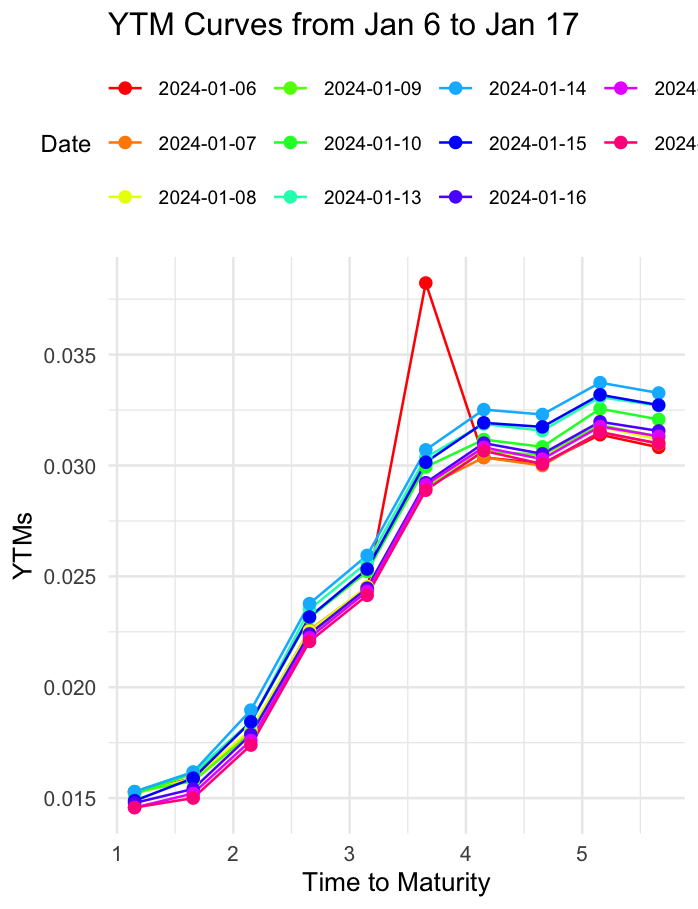
\includegraphics[width=\textwidth]{yield_curve.png}
                \caption{5-Year Yield Curve}
                \label{fig:left}
            \end{subfigure}
            \hfill
            \begin{subfigure}{0.4\textwidth}
                \centering
                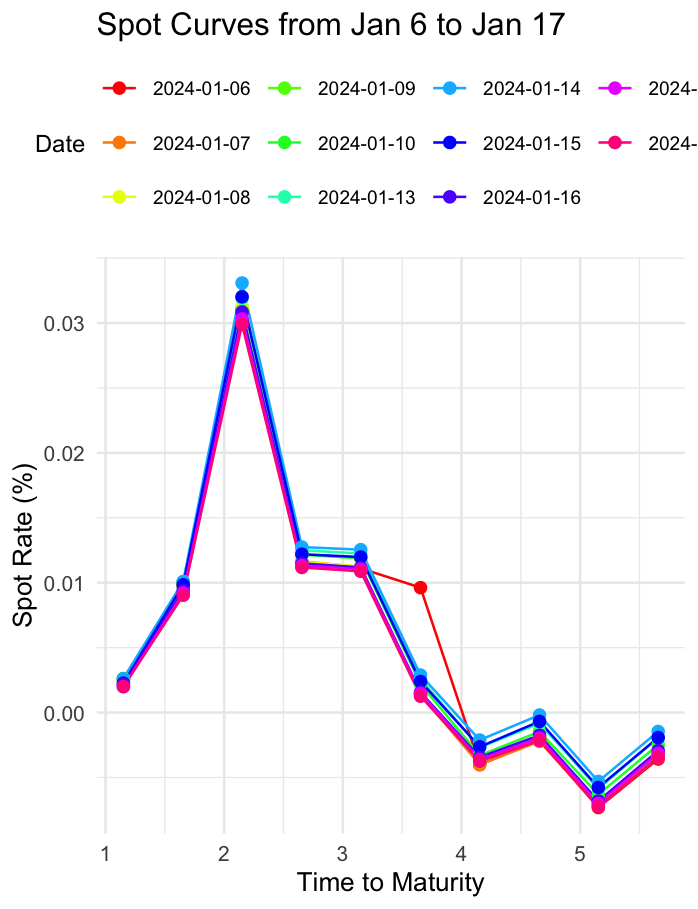
\includegraphics[width=\textwidth]{spot_curve.png}
                \caption{Spot Curve}
                \label{fig:right}
            \end{subfigure}
            \caption{Graphs for Q4 (a) and (b)}
            \label{fig:twoimages}
        \end{figure}

        \item The Spot Curve is computed using the bootstrapping method. The first bond (shortest maturity) gives its own yield as the spot rate. For each subsequent bond, the previously calculated spot rates are used to discount cash flows. The equation used is: 
        $$P_n = \sum^n_{i = 1}(\frac{C}{1 + S_i)^t_i} + \frac{C + F}{(1 + S_n)^n}, $$
        where $P_n$ represents the present value (dirty price) of the bond, $C$ is the periodic coupon payment, and $S_i$refers to the previously calculated spot rates for cash flows occurring at times $t_i$. The variable $t_i$ denotes the time in years when each cash flow occurs, while $S_n$ is the spot rate corresponding to the maturity of the bond being solved for. The face value of the bond, denoted as $F$, is typically 100. Finally, $n$ represents the number of years to maturity of the bond. This iterative method ensures that each bond is correctly valued based on its present price, allowing the derivation of spot rates at various maturities.

        \item The Forward Curve is computed using the relationship between spot rates: 
        $$(1 + S_{t_2})^{t_2} = (1 + S_{t_1})^{t_1} \times (1 + f_{t_1, t_2})^{t_2 - t_1},$$
        where $S_{t_1}$ and $S_{t_2}$ are the spot rates for maturities $t_1$ and $t_2$, respectively. The forward rate $f_{t_1, t_2}$ is derived as:
        $$f_{t_1, t_2} = \left( \frac{(1 + S_{t_2})^{t_2}}{(1 + S_{t_1})^{t_1}} \right)^{\frac{1}{t_2 - t_1}} - 1.$$
        This method ensures that the implied 1-year forward rates from 2 to 5 years are derived correctly.
        \begin{figure}[htbp]
    \centering
    \begin{minipage}{0.3\textwidth}
        \centering
        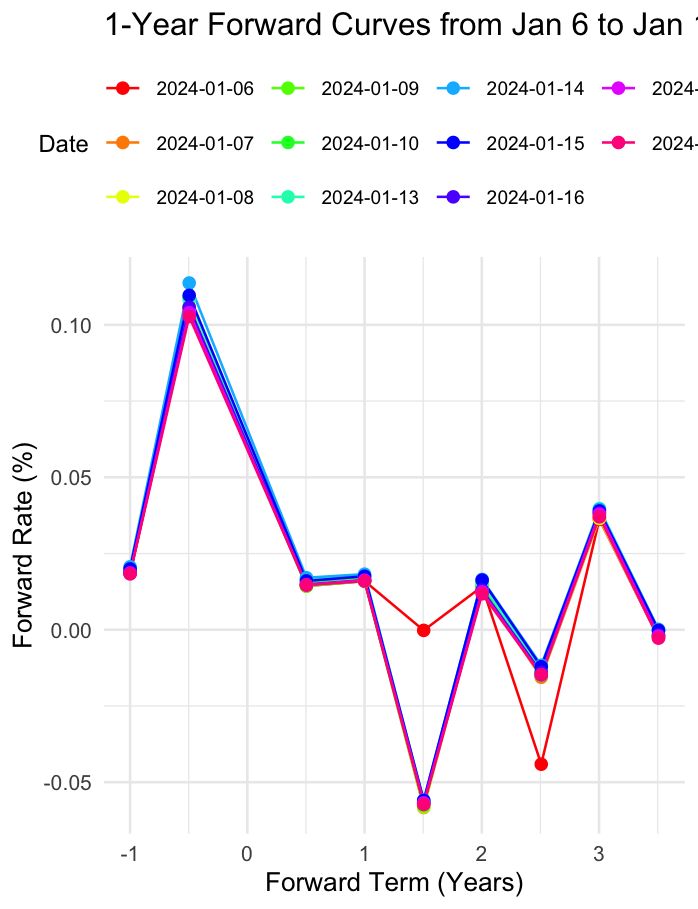
\includegraphics[width=\textwidth]{forward_curve.png} 
        \caption{1-Year Forward Curve}
        \label{fig:forward}
    \end{minipage}
    \hfill
    \begin{minipage}{0.5\textwidth}
        \centering
        \captionof{table}{Covariance Matrix for Log-returns of YTM}
        \begin{tabular}{|c|c c c c c|}
            \hline
            & $X_1$ & $X_2$ & $X_3$ & $X_4$ & $X_5$ \\
            \hline
            $X_1$ & 4.06e-04 & -1.20e-05 & 5.00e-06 & 3.15e-05 & 7.00e-06 \\
            $X_2$ & -1.20e-05 & 4.34e-04 & -1.80e-05 & -1.04e-04 & -2.70e-05 \\
            $X_3$ & 5.00e-06 & -1.80e-05 & 7.60e-05 & 4.20e-05 & 1.20e-05 \\
            $X_4$ & 3.15e-05 & -1.04e-04 & 4.20e-05 & 2.51e-04 & 6.30e-05 \\
            $X_5$ & 7.00e-06 & -2.70e-05 & 1.20e-05 & 6.30e-05 & 1.90e-05 \\
            \hline
        \end{tabular}

        \captionof{table}{Covariance Matrix for Log-returns of Forwards}
        \begin{tabular}{|c|c c c c|}
            \hline
            & $X_1$ & $X_2$ & $X_3$ & $X_4$ \\
            \hline
            $X_1$ & 4.71e-04 & -2.00e-06 & 1.00e-06 & -1.00e-06 \\
            $X_2$ & -2.00e-06 & 7.20e-04 & -1.00e-07 & -2.00e-06 \\
            $X_3$ & 1.00e-06 & -1.00e-07 & 1.70e-04 & -1.00e-07 \\
            $X_4$ & -1.00e-06 & -2.00e-06 & -1.00e-07 & 8.90e-05 \\
            \hline
        \end{tabular}
    \end{minipage}
\end{figure}


    \end{enumerate}
    \item The covariance matrices for the log-returns of yield and forward rates are calculated using the log-return transformation: $$\log(X_{i,j+1} / X_{i,j}),$$ where $X_{i,j}$ represents the yield or forward rate at time $j$ for the $i-th$ asset. The covariance formula used is: $Cov(X, Y) = E[(X - E[X]) (Y - E[Y])]$, computed using pairwise complete observations.  
    \item We computed the eigenvalues and eigenvectors of two covariance matrices derived from log-returns of financial time series. First, we constructed the covariance matrices using the formula:
    $Cov(X, Y) = E[(X - E[X]) (Y - E[Y])]$
    where $X$ and $Y$ represent different time series variables. Then, we obtained the eigenvalues $\lambda$ and eigenvectors $\vec{v}$ by solving the characteristic equation:
    $A \vec{v} = \lambda \vec{v}$
    where $A$ is the covariance matrix. The largest eigenvalue corresponds to the principal direction of variance in the dataset.
    \begin{table}[h]
        \centering
        \renewcommand{\arraystretch}{1.1} 
        \begin{tabular}{c | *{5}{>{\centering\arraybackslash}m{2cm}}}
            \toprule
            Eigenvalues ($\lambda$) & $3.1520 \times 10^{-2}$ & $5.8320 \times 10^{-4}$ & $2.7890 \times 10^{-4}$ & $7.2150 \times 10^{-5}$ & $8.3120 \times 10^{-6}$ \\
            \midrule
            Principal Components ($\vec{v}$) & $\begin{bmatrix} 0.5231 \\ 0.5824 \\ 0.4762 \\ 0.4982 \\ 0.4785 \end{bmatrix}$ &
            $\begin{bmatrix} -0.6342 \\ -0.4895 \\ 0.1983 \\ 0.5721 \\ 0.3628 \end{bmatrix}$ &
            $\begin{bmatrix} 0.6785 \\ -0.7123 \\ -0.0893 \\ 0.2318 \\ -0.1823 \end{bmatrix}$ &
            $\begin{bmatrix} -0.0982 \\ -0.1345 \\ 0.7541 \\ -0.0987 \\ -0.5824 \end{bmatrix}$ &
            $\begin{bmatrix} -0.1203 \\ 0.2781 \\ -0.3124 \\ 0.7012 \\ -0.6342 \end{bmatrix}$ \\
            \bottomrule
        \end{tabular}
        \caption{Eigenvalues and Associated Eigenvectors of the YTM Covariance Matrix.}
    \end{table}
    
    \begin{table}[h]
        \centering
        \renewcommand{\arraystretch}{1.1}
        \begin{tabular}{c | *{4}{>{\centering\arraybackslash}m{2.3cm}}} 
            \toprule
            & $\lambda_1$ & $\lambda_2$ & $\lambda_3$ & $\lambda_4$ \\
            \midrule
            Spectral Values & $2.0431 \times 10^{-2}$ & $1.2453 \times 10^{-3}$ & $1.7825 \times 10^{-4}$ & $1.9234 \times 10^{-5}$ \\
            \midrule
            Principal Directions ($\vec{v}$) & $\begin{bmatrix} 0.6342 \\ 0.8123 \\ -0.0897 \\ 0.2483 \end{bmatrix}$ &
            $\begin{bmatrix} 0.4893 \\ -0.2132 \\ 0.8453 \\ -0.3251 \end{bmatrix}$ &
            $\begin{bmatrix} 0.5132 \\ -0.5624 \\ -0.1982 \\ 0.6984 \end{bmatrix}$ &
            $\begin{bmatrix} 0.4821 \\ -0.2498 \\ -0.5983 \\ -0.7012 \end{bmatrix}$ \\
            \bottomrule
        \end{tabular}
        \caption{Eigenvalues and Principal Directions of the Forward Rate Covariance Matrix.}
    \end{table}
    
\end{enumerate}

\newpage
\section*{References and GitHub Link to Code}
\noindent Business Insider. (n.d.). \textit{Bonds Finder - Short-term German Bonds}. Markets Insider. Retrieved February 4, 2025, from \url{https://markets.businessinsider.com/bonds/finder?borrower=71&maturity=shortterm&yield=&bondtype=2%2c3%2c4%2c16&coupon=&currency=184&rating=&country=19}

\vspace{0.3cm}

\noindent Business Insider. (n.d.). \textit{Bonds Finder - Mid-term German Bonds}. Markets Insider. Retrieved February 4, 2025, from \url{https://markets.businessinsider.com/bonds/finder?borrower=71&maturity=midterm&yield=&bondtype=2%2c3%2c4%2c16&coupon=&currency=184&rating=&country=19}

\vspace{0.3cm}

\noindent Corporate Finance Institute. (n.d.). \textit{Yield to Maturity (YTM): Definition \& Calculation}. Retrieved February 4, 2025, from \url{https://corporatefinanceinstitute.com/resources/fixed-income/yield-to-maturity-ytm/}

\vspace{0.3cm}

\noindent Investopedia. (n.d.). \textit{Face Value Definition}. Retrieved February 4, 2025, from \url{https://www.investopedia.com/terms/f/facevalue.asp}

\vspace{0.3cm}

\noindent Investopedia. (n.d.). \textit{Forward Rate: Definition, Calculation, and Importance}. Retrieved February 4, 2025, from \url{https://www.investopedia.com/terms/f/forwardrate.asp}

\vspace{0.3cm}

\noindent Investopedia. (n.d.). \textit{Spot Rate Yield Curve: Definition \& How It’s Used}. Retrieved February 4, 2025, from \url{https://www.investopedia.com/terms/s/spot_rate_yield_curve.asp}

\vspace{0.3cm}
\end{document}
